\documentclass{elsarticle}
%\VignetteIndexEntry{Introduction to paleofire}
%\VignettePackage{paleofire}

%% Redefines the elsarticle footer
\makeatletter
\def\ps@pprintTitle{%
\let\@oddhead\@empty
\let\@evenhead\@empty
\def\@oddfoot{\it \hfill\today}%
\let\@evenfoot\@oddfoot}
\makeatother


\usepackage{natbib}
\bibliographystyle{elsarticle-harv}
\usepackage{graphicx}
\usepackage{lineno}
\usepackage{subfigure}
\usepackage[pdftex, colorlinks]{hyperref}
\usepackage{amsmath, amsfonts}  % extended mathematics
\usepackage{booktabs} % book-quality tables
\usepackage{units}    % non-stacked fractions and better unit spacing
\usepackage{multicol} % multiple column layout facilities
\usepackage{lipsum}   % filler text
\usepackage{fancyvrb} % extended verbatim environments
\fvset{fontsize=\normalsize}% default font size for fancy-verbatim environments
\usepackage{xspace}
\usepackage[utf8]{inputenc} 
\usepackage{mathtools}
\usepackage{etaremune}
\usepackage{url}
\usepackage{paralist}
\DeclareUnicodeCharacter{00A0}{ }
\DeclareRobustCommand{\ttfamily}{\fontencoding{T1}\fontfamily{lmtt}\selectfont}


%% optionally set the margins 
% \textwidth 6.75in
% \oddsidemargin -0.15in
% \evensidemargin -0.15in
% \textheight 9in
% \topmargin -0.5in
\newcommand{\ud}{\mathrm{d}}

% should be able to set figure size with:
%  <<label=test, fig=TRUE, width=5, height=5>>=

%-------------------------------------------------------------------------------
\RequirePackage{fancyvrb}
\RequirePackage{listings}
%-------------------------------------------------------------------------------
%-------------------------------------------------------------------------------
\usepackage{Sweave}



\begin{document}
\input{paleofire-paper-concordance}
\biboptions{authoryear,comma,round}



\begin{frontmatter}

\title{\texttt{paleofire}: an R package to analyse sedimentary charcoal records from the Global Charcoal Database to reconstruct past biomass burning}
\tnotetext[t1]{paleofire package version 1.1.3}
\tnotetext[t2]{Citing this vignette: Blarquez, O., Vannière, B., Marlon, J. R., Daniau, A. L., Power,M. J., Brewer, S., & Bartlein, P. J. (2014). paleofire: an R package to analyse sedimentary charcoal records from the Global Charcoal Database to reconstruct past biomass burning. Computers & Geosciences, 72, 255-261.}

\author[1,2]{Blarquez, Olivier\corref{cor1}}
\ead{blarquez@gmail.com}
\cortext[cor1]{Corresponding author}

\author[3]{Vannière, Boris}

\author[4]{Marlon, Jennifer R.}

\author[5]{Daniau, Anne-Laure}

\author[7]{Power, Mitchell J.}

\author[8]{Brewer, Simon}

\author[9]{Bartlein, Patrick J.}

\address[1]{Centre d'étude de la Forêt, Université du Québec à Montréal, Montréal, Québec, Canada}

\address[2]{Natural Sciences and Engineering Research Council of Canada Industrial Chair in Sustainable Forest Management, Forest Research Institute, Université du Québec en Abitibi-Témiscamingue, Rouyn-Noranda, Québec, Canada}

\address[3]{Centre National de la Recherche Scientifique (CNRS), UMR Chrono-Environment, Besançon, France}

\address[4]{Yale School Forestry and Environmental Studies, Yale University, New Haven, Connecticut, USA}

\address[5]{Centre National de la Recherche Scientifique (CNRS), Environnements et Paléoenvironnements Océaniques et Continentaux (EPOC), Unité Mixte de Recherche (UMR) 5805, Université de Bordeaux, Talence, France}

\address[7]{Natural History Museum of Utah and Department of Geography, University of Utah, Salt Lake City, Utah, USA}

\address[8]{Department of Geography, University of Utah, Salt Lake City, Utah, USA}

\address[9]{Department of Geography, University of Oregon, Eugene, Oregon, USA}




\begin{abstract}
We describe a new \texttt{R} package, \texttt{paleofire}, for analysis and synthesis of charcoal time series, such as those contained in the Global Charcoal Database (GCD),  that are used to reconstruct paleofire activity (past biomass burning). \texttt{paleofire} is an initiative of the Global Paleofire Working Group core team (www.gpwg.org), whose aim is to encourage the use of sedimentary charcoal series to develop regional-to-global syntheses of paleofire activity, and to enhance access to the GCD data by providing a common research framework. Currently, \texttt{paleofire} features are organized into three different parts related to (i) site selection and charcoal series extraction from the GCD; (ii) charcoal data transformation; and (iii) charcoal series compositing and synthesis. We provide a technical description of \texttt{paleofire} and describe some new implementations such as the circular block bootstrap procedure. We tested the software using GCDv3 data from eastern North America, and provide examples of interpreting results of regional and global syntheses.
\end{abstract}

\begin{keyword}
charcoal, fire, biomass burning, databases, \texttt{R} statistical language
\end{keyword}


\end{frontmatter}

\tableofcontents


%% main text
\section{Introduction}

In the last decade, regional and global syntheses of sedimentary charcoal records have been used to examine broad-scale patterns in palaeofire activity \citep{Carcaillet2002,Power2008,Daniau2012}. The linkages among fire, climate, vegetation and humans at centennial-millennial timescales have likewise been examined using global and regional syntheses \citep{Marlon2008, Ali2012}. Syntheses of charcoal records can also aid the validation and calibration of fire simulations \citep{Flannigan2001,Pechony2009,Girardin2013,Brucher2014}. Because fire influences ecosystems at all spatio-temporal scales (ranging from days to centuries and from microsites to biomes), a growing interest in paleofire research has emerged. Additionally, future wildfire regimes may have no analogues from recent decades, and so identifying reference conditions and baselines in the past has become crucial to projecting future wildfire activity \citep{Girardin2013}. Sedimentary charcoal series from individual sites are distributed worldwide, and are increasingly included in the Global Charcoal Database \citep[GCD]{Power2010}, which provides the scientific community a global charcoal dataset for research and archiving for sedimentary records of fire (the GCD is available at \url{http://gpwg.org/gpwgdb.html}). Syntheses of spatio-temporal changes in fire at global \citep{Marlon2008, Power2008, Daniau2012, Marlon2013} and regional \citep{Marlon2009, Mooney2011, Vanniere2011, Power2013} scales were obtained by applying several analytical steps implemented by a set of Fortran programs (Bartlein, P. J. unpublished). Because these statistical methods are not easily usable or modifiable, the Global Paleofire Working Group core team has developed a package using the open-source \texttt{R} statistical programming language. The new package should increase accessibility to paleofire data while providing the fire-science community with new analytical tools that include and extend the previously used functions for GCD data extraction and statistical analysis.
\\
The aim of this paper is to describe the \texttt{paleofire} \texttt{R} package that facilitates the analysis of charcoal records contained in the GCD. The \texttt{paleofire} package functions are organized into three parts: 
(i) GCD site selection and data extraction using a variety of criteria (geographic, sedimentary, etc.), (ii) charcoal data transformation, including re-scaling, single-record variance homogenization and nonparametric trend estimation and (iii) data synthesis, including confidence limit estimation using resampling procedures.


\section{Global Charcoal Database to paleofire data synthesis}

The \texttt{paleofire} package works in conjunction with the \texttt{GCD} \texttt{R} package that contains a simplified version of the charcoal dataset in order to accommodate the different update frequency between the  \texttt{paleofire} package (frequent updates) and the Global Charcoal Database (infrequent updates). The \texttt{checkGCDversion()} function can be used to determine whether the \texttt{GCD} data package is current. If it is not, the function asks whether the user wants to update the data. The minimal package version numbers required for running the examples presented in this study are 1.1.3 and 3.0.3 for the \texttt{paleofire} and \texttt{GCD} packages respectively. Backward compatibility will be ensured from these versions.\\
As of \today, the GCD v3.0.3 contains a total of 736 charcoal records and is provided as a Microsoft Access database available at \url{http://gpwg.org}. The \texttt{GCD} data package is a simplified and reduced version of the GCD database. The package consists of two data frames containing site metadata and charcoal data. The two data frames combine several tables from the GCD in order to simplify analysis in \texttt{R}, and exclude chronology development information, such as radiocarbon dates; these will likely be added however in future releases.  
Although most analyses in \texttt{paleofire} may use data directly from the dataframes in the \texttt{GCD} package, it is also possible to analyze user-defined database extracts or other charcoal series not in the database using the pfAddData function. There is currently no mechanism for permanently adding data to the GCD package automatically; interested contributors should contact the GPWG instead.
The site metadata is accessible by typing the \texttt{data(paleofiresites)} command at the \texttt{R} prompt. This data frame provides a unique identifier for each site in the id\_site column and associated metadata such as chronological, sedimentary or geographical information. 

The raw charcoal data are accessible with the \texttt{data(paleofiredata)} command. The data consist of a seven column data frame containing: (i) site unique identifier, (ii) sample depth, (iii) sample age, (iv) sample charcoal value, (v) sample charcoal unit, (vi) extraction method (sieved charcoal, pollen slide charcoals, etc.) and (vii) sample type unit (influx or concentration). The default setting for the \texttt{R} package is to select the preferred units (e.g., concentration or influx values are typically preferred over charcoal-to-pollen ratios if both are available) used in previous analysis \citetext{see \citealp{Daniau2012} or \citealp{Power2008}},  however \texttt{paleofire} allows one to analyse charcoal records with user-defined units or methods (e.g. sieved \textit{vs} pollen slide charcoals, see pfSiteSel and pfTransform functions help for details).  

\section{Technical description of \texttt{paleofire}}

Here we provide a technical description and several illustrative examples of \texttt{paleofire}. The \texttt{paleofire} package is written in the \texttt{R} scientific computing language (\texttt{R} Development Core Team, 2011) and was developed under the \texttt{R} 3.0.3 version but remains compatible with \texttt{R} >=2.10.0. The functions in \texttt{paleofire} are arranged into three groups associated with data selection, charcoal series transformation, and synthesis. We used the S3 method scheme to implement generic plotting and summary functions.

To present some of the \texttt{paleofire} capabilities, the examples below use charcoal series from Eastern North America. For additional examples and a detailed overview of individual functions, the reader is referred to the online help available at \url{http://cran.r-project.org/web/packages/paleofire/paleofire.pdf}.

\subsection{Site selection}

Two functions are dedicated to site selection. The first one, \texttt{pfInteractive} requires users to interactively draw a polygon on a map to select sites with respect to their geographic location. The function returns a list object containing site names and identifiers that is further used in the following analysis steps and is called using \texttt{pfInteractive()}.


\begin{Schunk}
\begin{Sinput}
> #install.packages("paleofire",repo="http://cran.r-project.org")
> library(paleofire)
\end{Sinput}
\end{Schunk}


The \texttt{pfSiteSel} function is more versatile than \texttt{pfInteractive} and has arguments for a variety of user-defined criteria. In the example below we select charcoal series between 30° and 90° latitude and -100° and -50° longitude, and include only those with at least one geochronological (\textsuperscript{14}C or \textsuperscript{210}Pb dating, tephra layer, etc.) control point each 2500 year. 

\begin{Schunk}
\begin{Sinput}
> ID <- pfSiteSel(lat>30 & lat<90, long>-100 & long<(-50), 
+                 date_int<=2500)
> length(ID$id_site)
\end{Sinput}
\begin{Soutput}
[1] 71
\end{Soutput}
\end{Schunk}

Seventy-one sites are selected and stored in the ID object of the class \texttt{pfSiteSel}. The summary function associated with the \texttt{pfSiteSel} object returns a table (Table SI1) containing site information, including geographic (latitude, longitude and elevation) and chronological descriptors (number of chronological control points, number of samples, minimum and maximum estimated ages). In the example below the \texttt{summary} function is applied to the ID object and the \texttt{pfSiteSel} function is used to select site records with at least 20 samples.

\begin{Schunk}
\begin{Sinput}
> sumID <- summary(ID)
> ID <- pfSiteSel(id_site %in% ID$id_site & num_samp>=20)
> length(ID$id_site)
\end{Sinput}
\begin{Soutput}
[1] 57
\end{Soutput}
\end{Schunk}


The 57 selected sites can be plotted on a map using the generic \texttt{plot} function ; a zoom level can be specified using the zoom argument. The use of this function is illustrated in the example below, which is used to construct Figure 1. The \texttt{plot} function may also be used to explore the sampling resolution of sites using the \texttt{type="chronology"} argument. 


\begin{figure*}
\centering
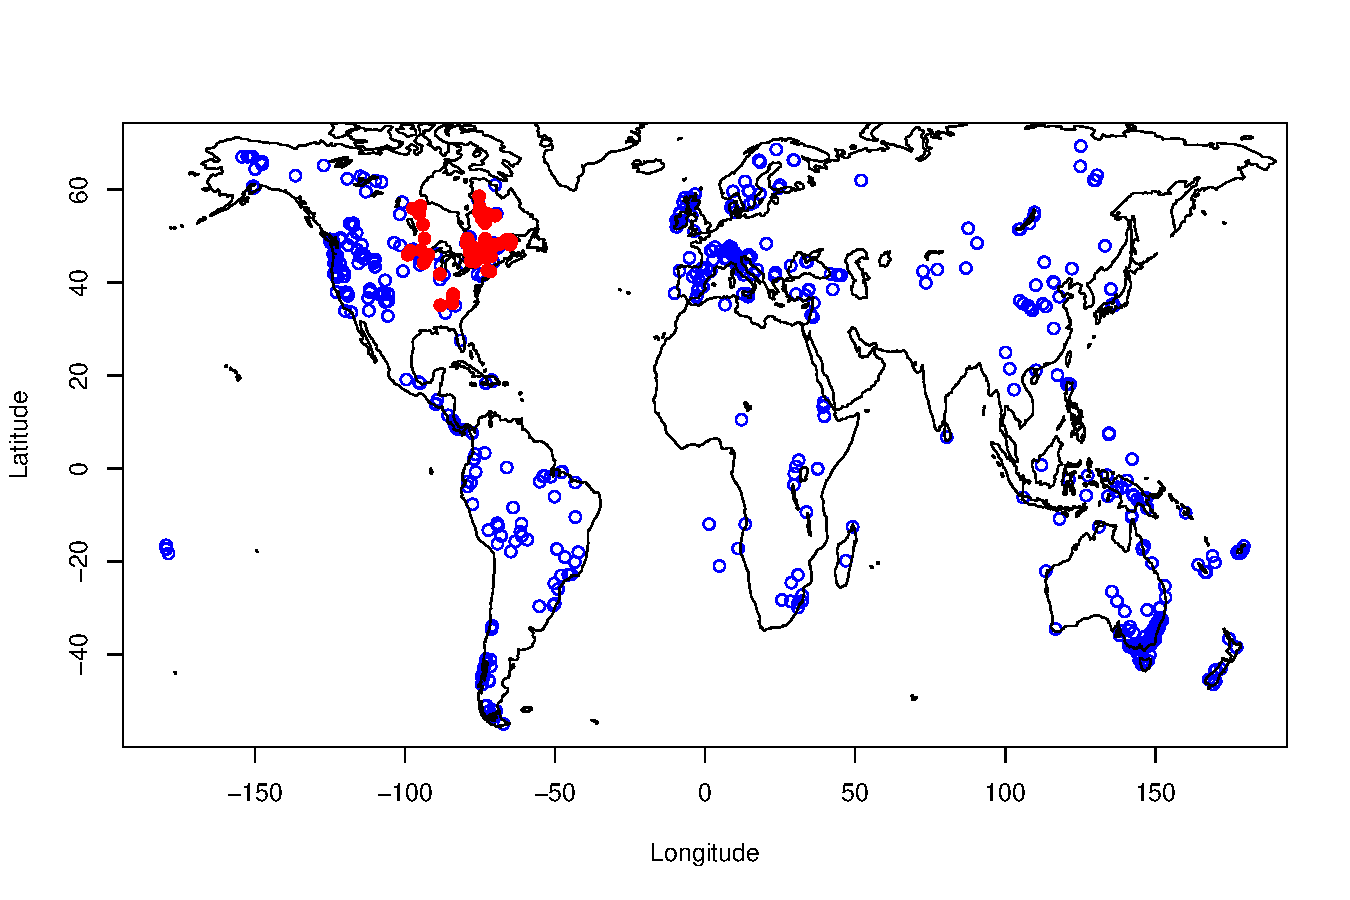
\includegraphics{paleofire-paper-fig1}

\caption{Location maps of selected North Eastern American charcoal sites from GCDv3 (a). The zoom argument was set to "world". Selected sites are displayed using filled red circles; unselected GCD sites are displayed using empty blue circles.}
\end{figure*}

\subsection{Data transformation}

Charcoal values contained in the GCD can vary widely among and within sites due to multiple factors. For instance, variations in (absolute) charcoal abundances can be related to different analytical methods \citetext{i.e. sediment treatment; \citealp{Tinner2003}} as well as to unique physiographic site characteristics \cite{Marlon2006}. Variations in charcoal values may also be linked to differences in the types of records \citetext{pollen slide charcoals, sieved charcoals, charcoal/pollen ratios, \citealt{Carcaillet2001a}}. Lastly, differences in the original sample quantities (influx, concentration, percentage) could also contribute to variations in charcoal values. Consequently, transformation and standardization of different charcoal records is a highly recommended step in generating a synthesis. A methodology to standardize charcoal records was proposed by \citet{Power2008} and involved a three-step data transformation including a minimax data-rescaling, variance homogenization using \citet{Box1964} data transformation, and a final rescaling to Z-scores. Using the \texttt{pfTransform} function these transformations are done on influx using the following command:

\begin{Schunk}
\begin{Sinput}
> TR1 <- pfTransform(ID, method=c("MinMax","Box-Cox","Z-Score"))
\end{Sinput}
\end{Schunk}


Note that by default the \texttt{pfTransform} function calculates influx for series whose data is given in concentrations, by multiplying concentrations by sediment vertical accretion rate ($cm.yr^{-1}$) calculated using the age-depth model for each record (the \texttt{QuantType="NONE"} argument can be passed to the \texttt{pfTransform} function for keeping original units but it is not recommended). The \texttt{method} argument may list single or multiple methods (that are computed in the same order as given in the function), relating to charcoal data transformation or smoothing. The distributions of charcoal values typically have long right tails, and can generally be easily transformed to a symmetrical “normal”-like distribution \cite{Higuera2011}.  The transformations we implemented include both the \citet{Box1964} parametric power transformation technique (default method) and the modified Box-Cox modulus transformation, proposed by \citet{John1980}, which is known to more effectively produce normality in long tailed data, i.e. in the case of charcoal series data presenting numerous zero values. These are accessible through the pfTransform function using the \texttt{type=c("BoxCox1964" , "JohnDraper")} argument. 

The types of filtering (smoothing or compositing) techniques implemented here include running means, median, min, max, quantiles, locally weighted scatter plot smoother (LOESS) and smoothing splines; all these methods take an additional parameter giving the window width for computations (RunWidth argument) or the smoothing parameter in the case of the LOESS or the smoothing-spline methods (span argument). Associated to \texttt{pfTransform} users may choose to add their own data to the analysis using the \texttt{pfAddData} function that uses the CharAnalysis file type format \cite[][freely available at \url{https://github.com/phiguera/CharAnalysis}]{Higuera2009}, or any file containing charcoal quantities and associated depth and age information as input. In the following example we will add the charcoal data from \citet{Senici2013}. The \texttt{BasePeriod} argument is used to set the period 200-4000 BP as a base period for the Z-score calculation \citep{Power2008}. Note that a minimax data-rescaling step was added after the Box-Cox transformation because Box-Cox transformed series are comparable only if they share identical $\lambda$ values \citep{Marlon2008}.



\begin{Schunk}
\begin{Sinput}
> ## Add Ben lake and Small lake data to the 
> # analysis (Senici et al., 2013) 
> download.file(url="http://blarquez.com/public/data/data_cageo.zip", 
+                 destfile="data_cageo.zip")
> unzip("data_cageo.zip")
> mydata=pfAddData(files=c("Ben.csv","Small.csv"), 
+                    metadata="metadata.csv", type="CharAnalysis")
> ## Transform:
> TR2 <- pfTransform(ID,add=mydata,BasePeriod=c(200,4000),
+                    method=c("MinMax","Box-Cox","MinMax","Z-Score"))
> ## Delete downloaded files
> file.remove(c("Ben.csv","Small.csv","data_cageo.zip","metadata.csv"))
\end{Sinput}
\end{Schunk}

\subsection{Data synthesis and compositing}

Synthesizing or compositing charcoal series typically involves pooling the different series in order to calculate the mean charcoal value (across sites) at each time step. This simple operation could be performed in different ways using the \texttt{pfComposite} function. Alternatively, a data-binning procedure can be used to calculate a composite curve. The binning sequence must be supplied in order to allow the \texttt{pfComposite} function to calculate the mean charcoal value for each series within each binning interval and then calculate the mean for all series. This can be achieved using arbitrary 500-year bin widths:

\begin{Schunk}
\begin{Sinput}
> COMP1 <- pfComposite(TR2, binning=TRUE, 
+                      bins=seq(from=0,to=11000, by=500))
\end{Sinput}
\end{Schunk}

This approach (\texttt{pfComposite}) is equivalent to \citet{Power2008} but \texttt{paleofire} also implements the methods proposed by \citet{Marlon2008} and \citet{Daniau2012}, which consists of a two-stage smoothing method (\texttt{pfCompositeLF}). The procedure implemented in the package was slightly modified compared to \citet{Marlon2008} but returns highly comparable results (see SI for details). The two-stage smoothing method first "pre-bins" individual charcoal series using non-overlapping bins in order to ensure that records with high sample resolution do not have a disproportionate influence on the composite record, and that data will be not interpolated for records with a lower resolution. The second step smooths the pre-binned series using a locally-weighted scatter plot smoother "LOWESS" \citep{Cleveland1979} with a pre-defined constant bandwidth (half-width) given in the years (\texttt{hw} argument). In the following example we will pre-bin the data with 20 year non-overlapping bins and a LOWESS smoother with a 500 year window half width (i.e., a 1000-year smoothing window).

\begin{Schunk}
\begin{Sinput}
> COMP2 <- pfCompositeLF(TR2, tarAge=seq(-50,12000,20), 
+                        binhw=10, hw=500, nboot=100)